This section provides mockups and general descriptions on the UI of the different client applications.

\subsection{User web browser client}
	The main mockups have already been presented in RASD \textit{section 3.2.1}.
	Follows an additional detail on the profile management view.

	\begin{figure}[h]
		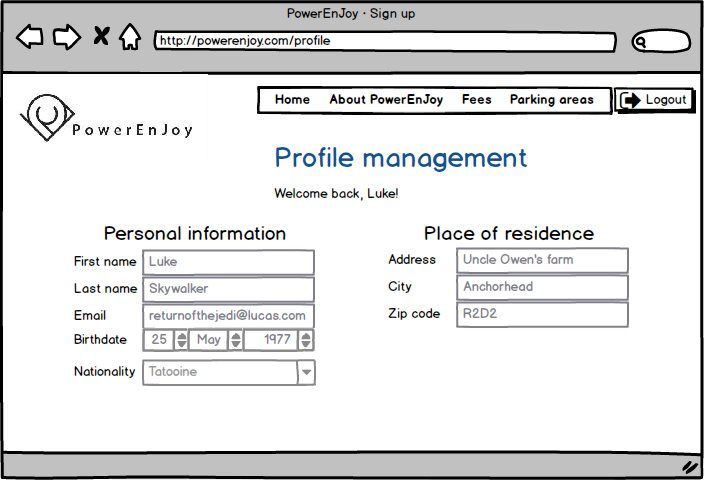
\includegraphics[width=\textwidth, center]{img/user_interface_design/Website_profile_management.png}
		\caption{User web browser client: profile management.}
	\end{figure}

\subsection{User mobile app client}
	The main mockups have already been presented in RASD \textit{section 3.2.1}.
	Follows a partial detail on the registration process though the mobile app. Because of the reduced dimension of the mobile device, part of the form is not displayed and is available scrolling down the page.
	In addition to this, the main section covering the emergency report opening is included.

	\begin{figure}[h]
		\begin{subfigure}{0.5\textwidth}
			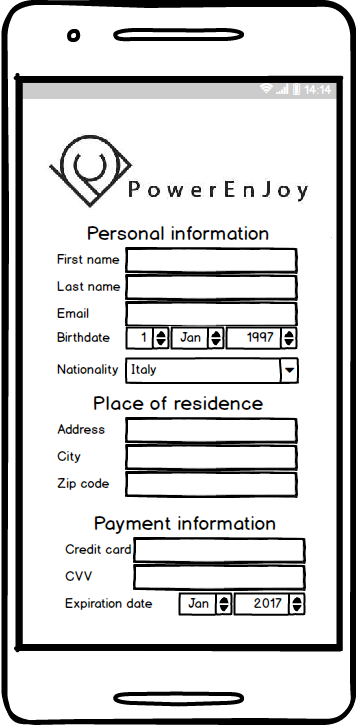
\includegraphics[width=0.5\textwidth, center]{img/user_interface_design/App_sign_up.png}
			\caption{User mobile app client: sign up.}
		\end{subfigure}
		\begin{subfigure}{0.5\textwidth}
			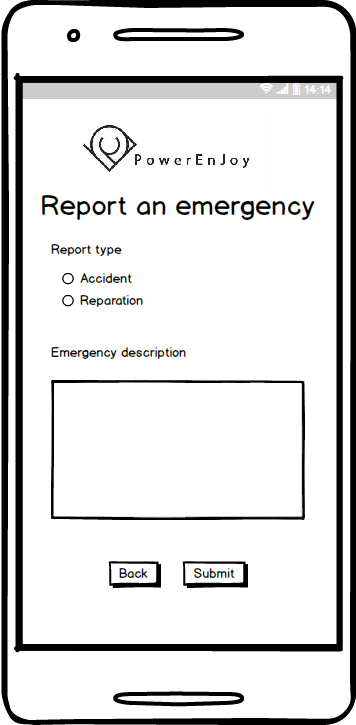
\includegraphics[width=0.5\textwidth, center]{img/user_interface_design/User_emergency_report.png}
			\caption{User mobile app client: emergency report.}
		\end{subfigure}
	\end{figure}
\FloatBarrier

\subsection{Car client}
	This application resides on the tablet permanently installed on the car. For this reason, the tablet does not allow the user to exit the application, which is always in full screen mode. The user interface of the app is designed to assist the user during the ride with useful information and allow him to open an emergency report.

	\begin{figure}[h]
		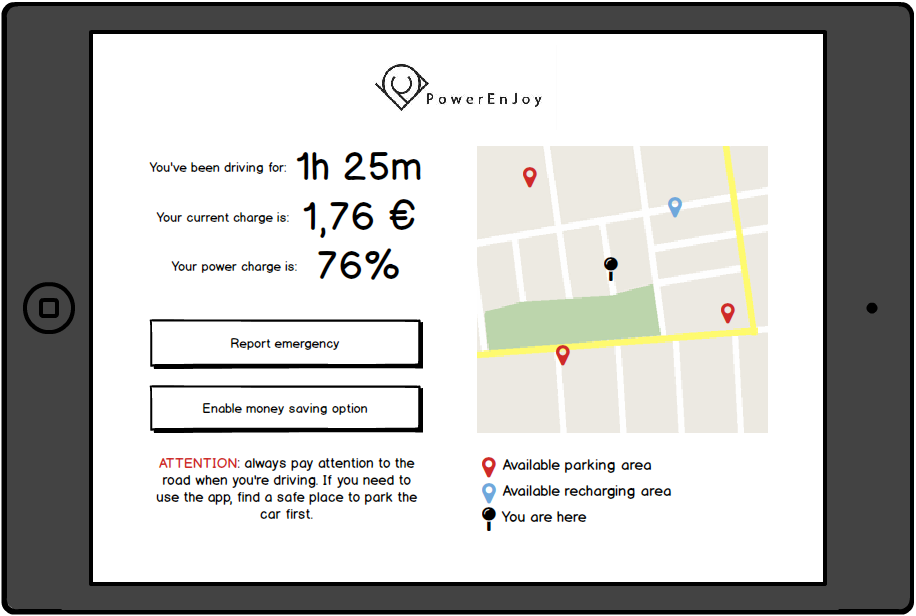
\includegraphics[height=0.4\textheight, center]{img/user_interface_design/Car_ride.png}
		\caption{Car client: ride.}
	\end{figure}
	\begin{figure}[h]
		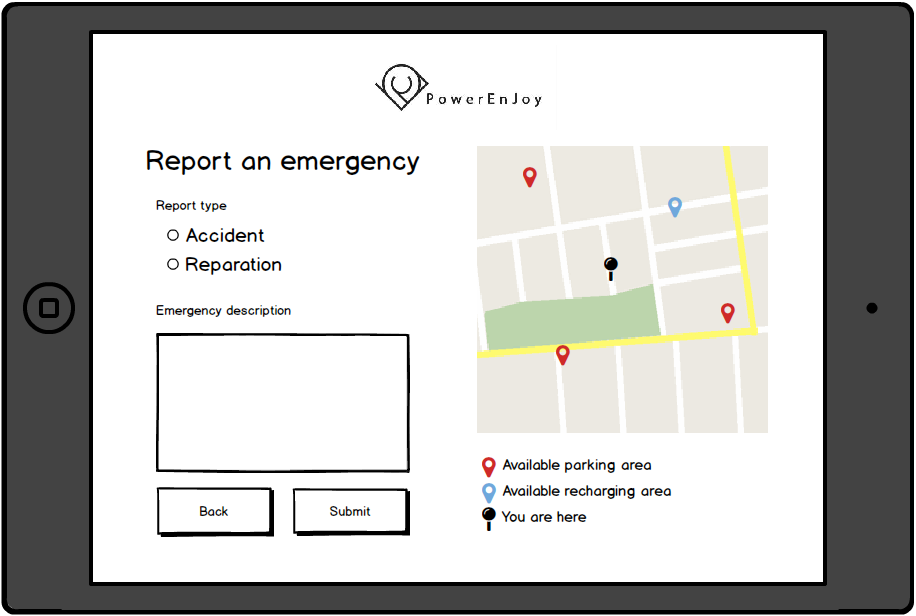
\includegraphics[height=0.4\textheight, center]{img/user_interface_design/Car_emergency_report.png}
		\caption{Car client: emergency report.}
	\end{figure}
\FloatBarrier

\subsection{Operator mobile client}
	The app provided to the operator is installed on the company tablet and is available to be used by the operator when he needs it. The app allows him to take a have an overview of the assigned emergency and to update its status gradually during the intervention. A report is attached for additional information.

	\begin{figure}[h]
		
\includegraphics[height=0.4\textheight, center]{img/user_interface_design/Operator_main.png}
		\caption{Car client: emergency report.}
	\end{figure}
\FloatBarrier

\subsection{Admin app client}
	From the designated application, the administrator has the possibility to modify the core parameters of the system and manage the dispatching of operators to the assistance requests.\newline
	A simple form view is dedicated to the parameter adjustment.\newline
	The operator dispatching functionality starts from an overview board, which summarizes the situation of the various assistance interventions on a map. For each assistance request, it is possible to visualize a small report or to open the detailed page. The latter, allows the actual dispatching of an operator for an open emergency, and provides general information about its status, displaying both the user's description of the problem and the operator's report on it.

	\begin{figure}[h]
		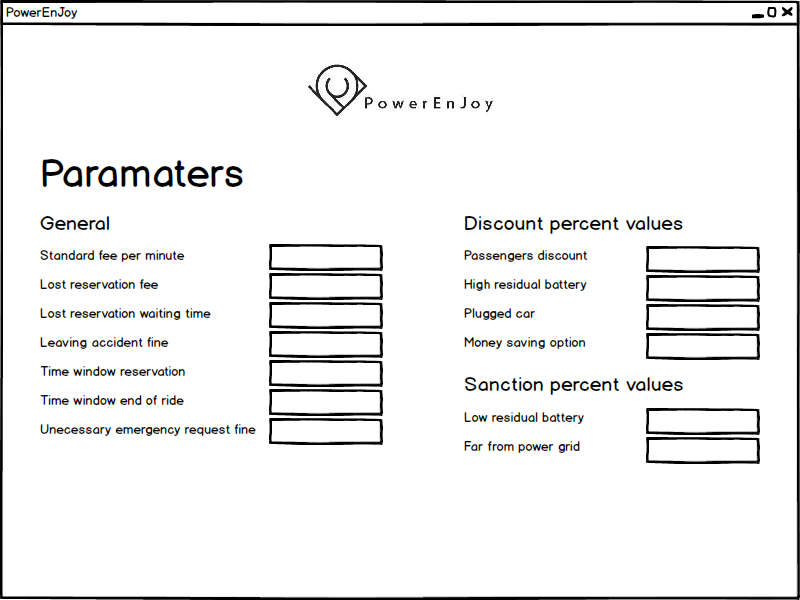
\includegraphics[height=0.4\textheight, center]{img/user_interface_design/Admin_parameters.png}
		\caption{Admin app client: parameters management.}
	\end{figure}
	\begin{figure}[h]
		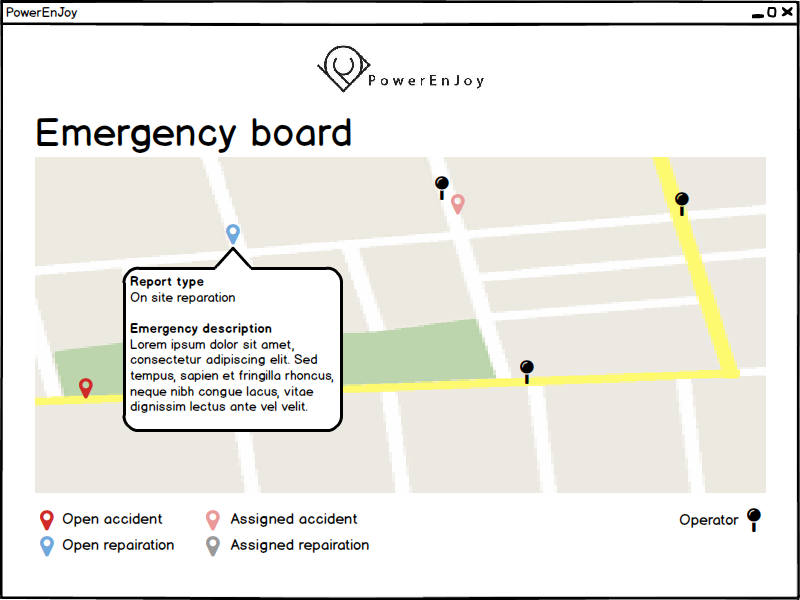
\includegraphics[height=0.4\textheight, center]{img/user_interface_design/Admin_emergency_board.png}
		\caption{Admin app client: operator dispatching main board.}
	\end{figure}
	\begin{figure}[h]
		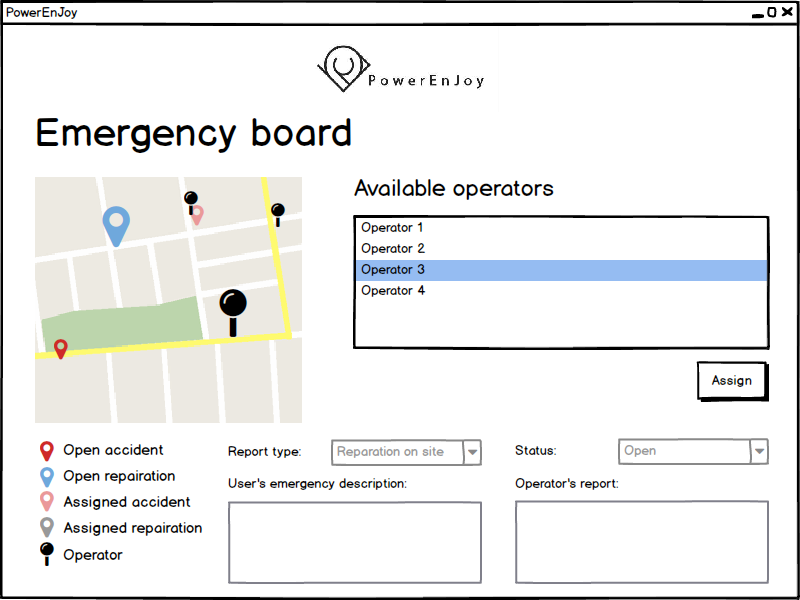
\includegraphics[height=0.4\textheight, center]{img/user_interface_design/Admin_emergency_detail.png}
		\caption{Admin app client: operator dispatching details.}
	\end{figure}
\FloatBarrier
